% LectureTemplate for ME3050 -  Dynamics Modeling and Controls - Tennessee Technological University
% Tristan Hill - Spring 2020 - Summer 2020 - Fall 2022
% Dynamics Modeling and Controls
% Lecture Module - Introduction - Topic 1  - What is System Dynamics? 

% Document settings

%\documentclass{beamer}                  % for presentation ?
\documentclass[handout]{beamer}  % for handout ?

\usepackage{/home/thill/Documents/lectures/dmc_lectures/dmc_lectures}


\newcommand{\MNUM}{1\hspace{2mm}} % Module number
\newcommand{\TNUM}{1\hspace{2mm}} % Topic number 
\newcommand{\moduletitle}{Introduction} % Titles and Stuff
\newcommand{\topictitle}{What is System Dynamics?} 

\newcommand{\sectiontitleI}{Welcome Back!} % More Titles and Stuff
\newcommand{\sectiontitleII}{Definition of Dynamics}
\newcommand{\sectiontitleIII}{Modeling and Analysis}
\newcommand{\sectiontitleIV}{Model Based Design}
\newcommand{\sectiontitleV}{Major Topic Covered }


\author{ME3050 - Dynamic Modeling and Controls}
\title{Module \MNUM - \moduletitle}
\date{Mechanical Engineering\vspc Tennessee Technological University}

\begin{document}

\lstset{language=MATLAB,basicstyle=\ttfamily\small,showstringspaces=false}

\frame{\titlepage \center\begin{framed}\Large \textbf{Topic \TNUM - \topictitle}\end{framed} \vspace{5mm}}

% Section 0 - Outline
\frame{
	
	\large \textbf{Topic \TNUM - \topictitle} \vspace{3mm}\\
	
	\begin{itemize}
	
		\item \sectiontitleI    \vspc % Section I
		\item \sectiontitleII 	\vspc % Section II
		\item \sectiontitleIII 	\vspc %Section III
		\item \sectiontitleIV 	\vspc %Section IV
		%\item \sectiontitleV 	\vspc %Section V
	
	\end{itemize}

}


% Section 1
\section{Welcome Back!}

\frame{
\frametitle{Welcome to New Video topics}
\large{\it Welcome Back!\vspace{3mm}\\}



}

% Section 2
\section{Definition of Dynamics}

\frame{
\frametitle{Definition of Dynamics}

\large
Dynamics is ...\vspcc

the study of how moving objects behave, \vspcc
or \vspcc
an area of mechanics that studies movement and its causes,\vspcc
or \vspcc
%\Large{"The dynamical system concept is a mathematical formalization for any fixed "rule" which describes the time dependence of a point's position in its ambient space. "} \vspace{5mm} \\

{\it system dynamics} is the study of {\bf modeling} and {\bf analysis} of dynamical systems as a function of time.\vspc



}

\frame{
\frametitle{Dynamics vs System Dynamics}

\large
Dynamics: find state of \underline{object} at \underline{a specific instant in time} \vspccc

System Dynamics: find state of \underline{system} as a \underline{function of time}  \vspc

$\rightarrow$ Leads to use of differential equations. $m\ddot{x}+c\dot{x}+kx=f(t)$

}

% Section 3
\section{Modeling and Analysis}

\frame{
\frametitle{What is Mathematical Modeling?}

A mathematical model is a description of a system using mathematical concepts and language. The process of developing a mathematical model is termed mathematical {\bf modeling} ... \vspc
...  used in the natural sciences and engineering disciplines ...  \href{https://en.wikipedia.org/wiki/Mathematical_model}{\tiny Wikipedia}

\begin{itemize}
\item Model Simplification
\item Force and Loading Analysis with FBDs
\item Fundamental Laws Lead to Equations of Motion
\item Newton's Second Law and Conservation of Energy

\end{itemize}

}

\frame{
\frametitle{What is Analysis?}

{\bf Analysis} is the process of breaking a complex topic or substance into smaller parts in order to gain a better understanding of it... \href{https://en.wikipedia.org/wiki/Analysis}{\tiny Wikipedia}

\begin{itemize}
\item Study Model to find System Response
\item Time-Domain analysis: examine system response in time to various inputs and initial conditions
\item Frequency-Domain analysis: examine system response when subject to sinusoidal inputs


\end{itemize}

}

% Section 4
\section{Model Based Design}

\frame{
\frametitle{Model Based Design}

Model-Based Design (MBD) is a mathematical and visual method of addressing problems associated with designing complex control, signal processing and communication systems. It is used in many motion control, industrial equipment, aerospace, and automotive applications... \href{https://en.wikipedia.org/wiki/Model-based_design}{\tiny Wikipedia}

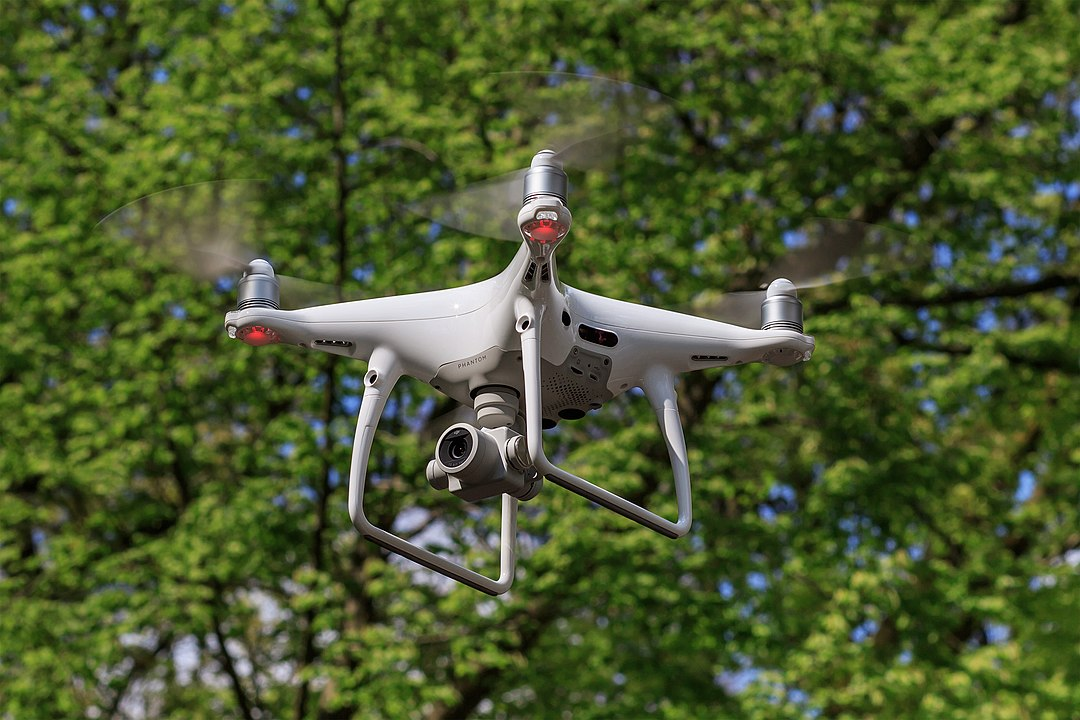
\includegraphics[scale=.08]{dji_phantom_fig2.jpg}\hspccc
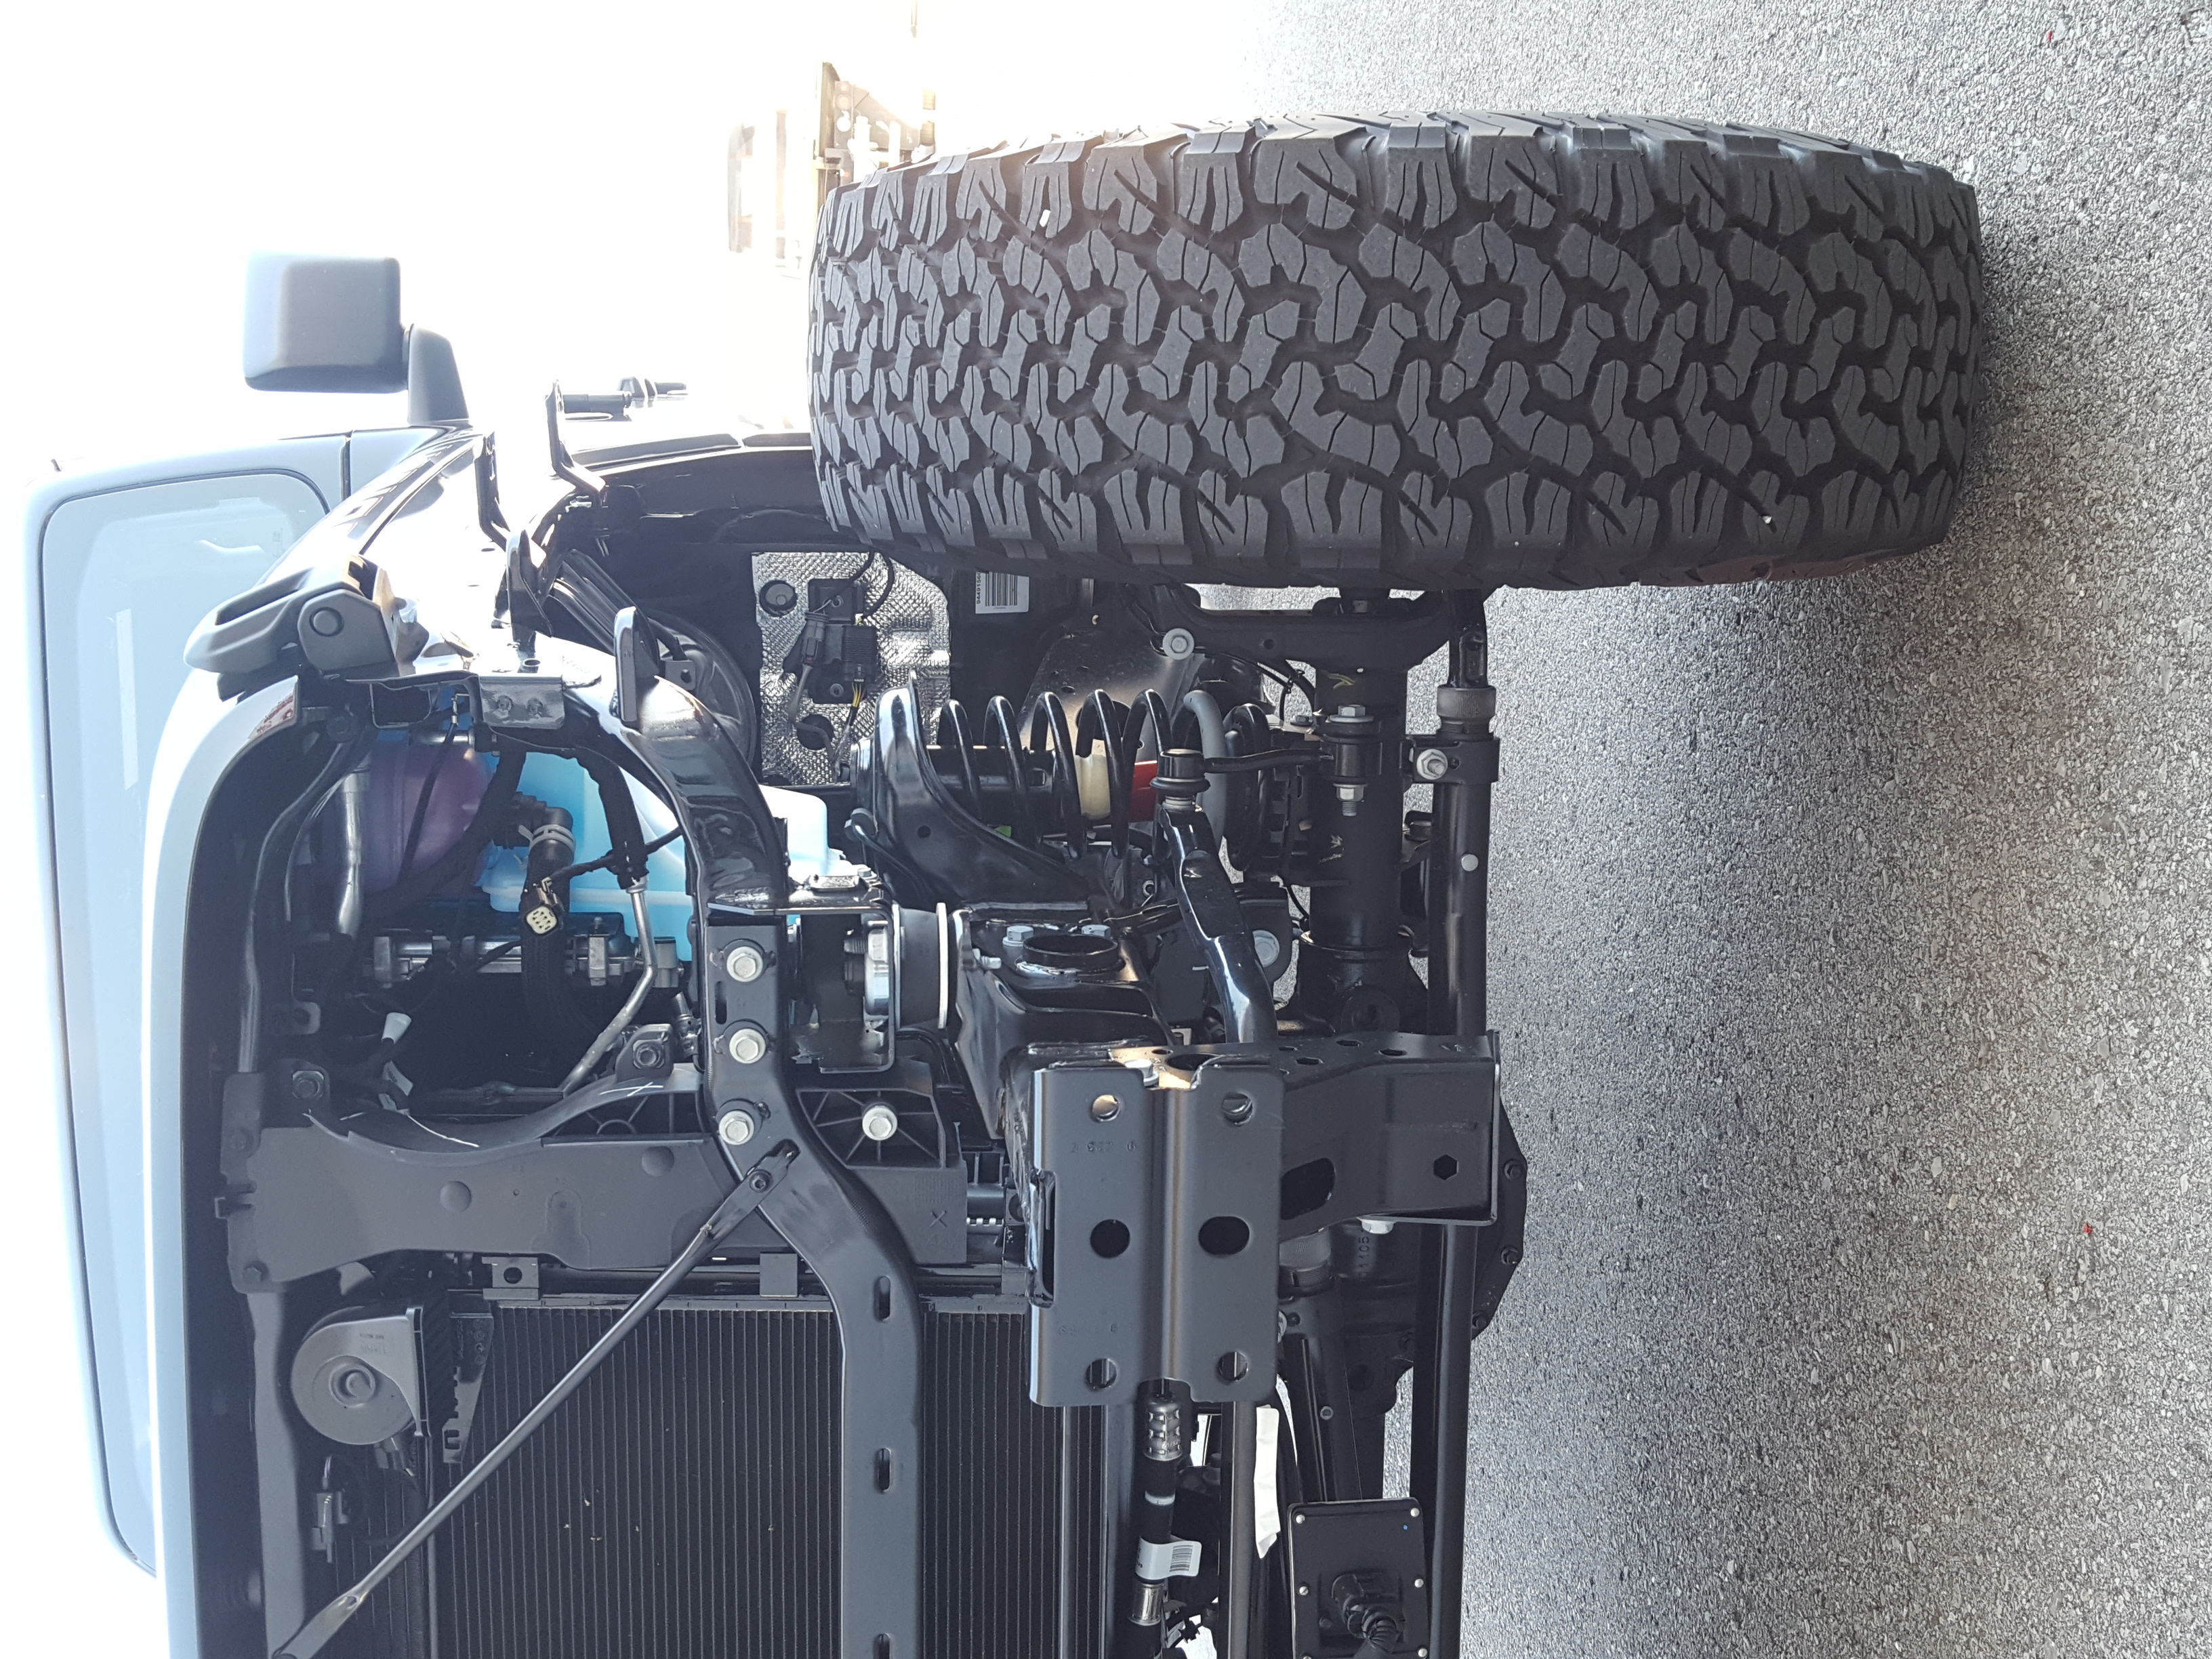
\includegraphics[scale=.025,angle=-90,origin=c]{jeep_01.jpg} \hspccc
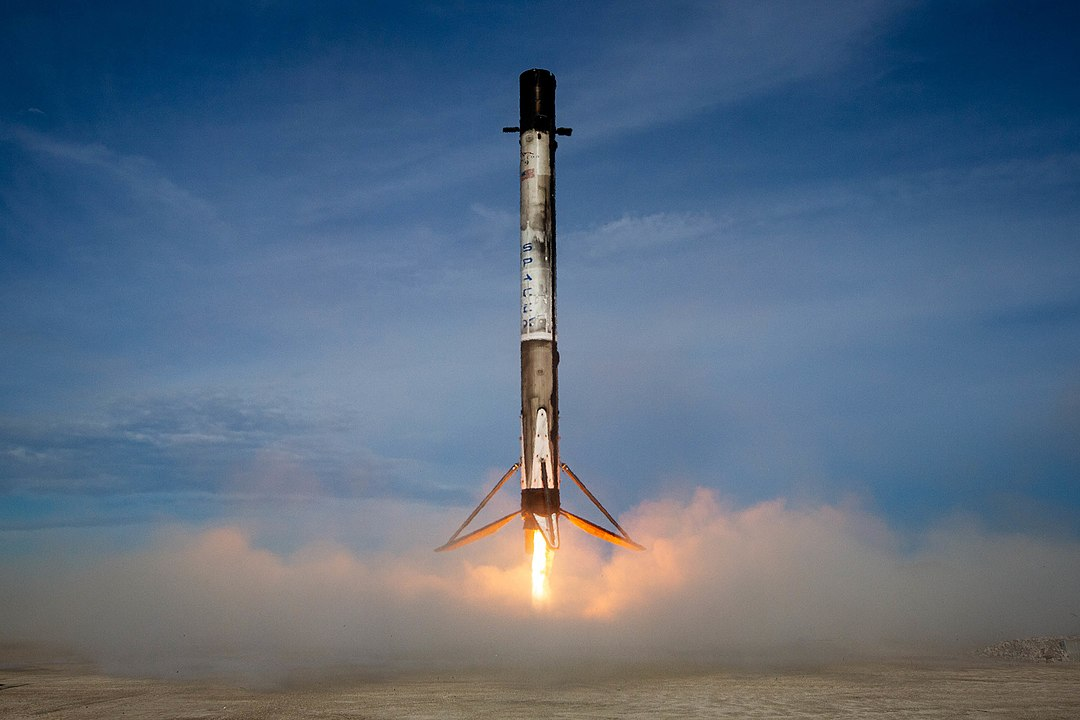
\includegraphics[scale=.1]{falcon9_fig2.jpg} \\
{\tiny\href{https://en.wikipedia.org/wiki/Phantom_(UAV)}{Image: Wikipedia} \hspace{20mm}Image: TH \hspace{20mm}\href{https://en.wikipedia.org/wiki/SpaceX\#/media/File:CRS-18_Mission_(48380511427).jpg}{Image: Wikipedia} }
}

\end{document}





